\scanpage{7}

soient alignés (p.ex les vecteurs .
\[
 (0,0,1,1)\quad(1,0,0,1)\quad(1,1,0,0)
\]
ne sont pas coplanaires \deleted{\unsure{les}} i.e la matrice
\[
 \begin{pmatrix}0&0&1&1\\1&0&0&1\\1&1&0&0\end{pmatrix}
 \quad\text{de rang }3\ \ldots)
\]

Donc ils forment une base projective de $P^2$, donc, \deleted{\unsure{$M_4\simeq$}} si $\Pi=(S,A)$ est un quadrilatère combinatoire, $\mathbb M(\Pi)$ s'identifie à l'enveloppe projective de $A$.

\figure{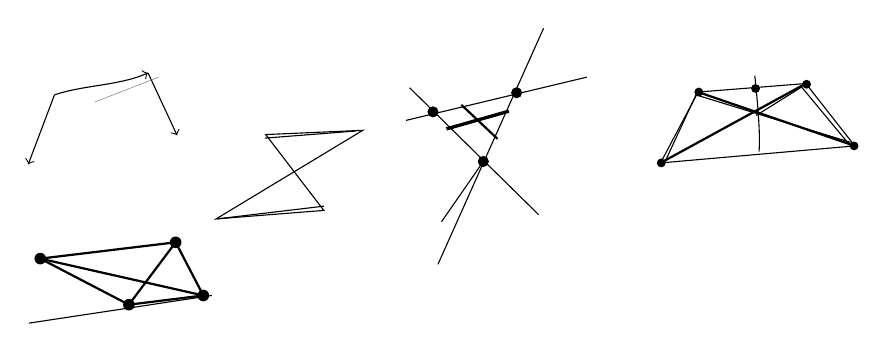
\begin{tikzpicture}[x=.009cm,y=-.009cm]
\draw[->] (149,990)--(112,1088);
\draw[->] (149,990)..controls(190,976)and(241,977)..(281,959);
\draw[->] (281,959)--(322,1047);
\draw[very thin,gray] (206,1000)--(296,965);
\draw (377,1165)--(584,1040)--(447,1046)--(529,1153)--cycle;
\draw[thin] (378,1165)--(529,1147) (446,1051)--(574,1041);
\draw (645,1026)--(900,965) (650,980)--(832,1159) (690,1229)--(839,896);
\draw (695,1169)--(754,1084); \draw[very thick] (702,1038)--(790,1013);
\draw[thick] (723,1004)--(774,1052);
\foreach \x/\y in {683/1014,801/987,754/1084}{\fill (\x,\y) circle(2pt);}
\draw (1004,1086)--(1057,986)--(1209,974)--(1278,1062)--cycle;
\draw[thick] (1004,1086)--(1209,974) (1057,986)--(1278,1062);
\draw (1137,963)..controls(1140,994)and(1145,1039)..(1143,1070);
\draw[thin] (1010,1085)--(1054,990)--(1272,1057) (1139,1019)--(1203,979)--(1271,1061);
\foreach \x/\y in {1005/1086,1058/986,1210/975,1277/1062,1138/981}{\fill (\x,\y) circle(1.6pt);}
\draw (113,1312)--(371,1273); \draw[thick] (129,1221)--(320,1198)--(359,1273)--(254,1286)--cycle;
\draw[thick] (129,1221)--(359,1273) (254,1286)--(320,1198);
\foreach \x/\y in {129/1221,320/1198,359/1273,254/1286}{\fill (\x,\y) circle(2.1pt);}
\end{tikzpicture}}
% archive sheet number: 13
